%----------------------------------------------------------------------------------------
%	SECTION 1.5
%----------------------------------------------------------------------------------------

\section{Closed Sets and Limit Points.}

\begin{definition}
    A subset $A$ of a topological space  $X$ is said to be  \textbf{closed} if
    $\com{X}{A}$ is open.
\end{definition}

\begin{example}
    \begin{enumerate}
        \item[(1)] Consider $[a,b] \subseteq \R$, we have that
            $\com{\R}{[a,b]}=(-\infty,a) \cup (b, \infty)$ which is open in
            $\R$. So  $[a,b]$ is closed.

        \item[(2)] In  $\R \times \R$, the set  $A=\{x \times y: x,y \geq 0\}$  (i.e
            the first quadtant of the plane) is closed, for $\com{\R \times
            \R}{A}=((- \infty,0) \times \R) \cup (\R \times (-\infty,0))$, which
            is open in $\R \times \R$.

        \item[(3)] Consider the finite complement topology $\Tc_f$ on a set  $X$. We
            have that  $\com{X}{X}=\emptyset \in \Tc_f$, so  $X$ is closed,
            similarly,  $\emptyset$ is also closed. Likewise, if  $A \subseteq
            X$ is a finite set, then  $\com{X}{A}$ is also finite, and hence $A$
            is also closed. Thus, we have that all the closed sets of  $\Tc_f$
            are those finite subsets of  $X$. As a consequence, this example also
            illustrates that sets can be both closed and open.

        \item[(4)] In the discrete topology  $2^X$, every open set is closed. This is
            another example where open sets are also closed sets.

        \item[(4)] Consider  $[0,1] \cup (2,3)$ in the subspace topology on $\R$. We
            have that  $[0,1]$ is open in the subspace topology on $\R$;
            $[0,1]=[0,1] \cup (2,3) \cap (-\frac{2}{3},\frac{3}{2})$, similarly,
            $(2,3)$ is also open. Now taking  $\com{[0,1] \cup
            (2,3)}{(2,3)}=[0,1]$, which is open, so $[0,1]$ is closed in the
            subspace topology on  $\R$, by the same reasoning, so is  $(2,3)$.
    \end{enumerate}
\end{example}

\begin{theorem}\label{1.6.1}
    Let $X$ be a topological space. Then:
         \begin{enumerate}
             \item[(1)] $\emptyset$ and  $X$ are closed.

             \item[(2)] Arbitrary intersections of closed sets are closed.

             \item[(3)] Finite unions of closed sets are closed.
        \end{enumerate}
\end{theorem}
\begin{proof}
    We have that $\com{X}{\emptyset}=X$ and  $\com{X}{X}=\emptyset$, both of
    which are open in  $X$, so they are also closed in  $X$. Now let
    $\{U_{\alpha}\}$ be a collection of closed sets of  $X$. We have that:
        \begin{equation*}
            \com{X}{\bigcap_{\alpha}}{U_{\alpha}}=\bigcup_{\alpha}{\com{X}{U_{\alpha}}}.
        \end{equation*}
        Similarly, for $\{U_i\}_{i=1}^{n}$, we have
        \begin{equation*}
            \com{X}{\bigcup_{i=1}^{n}}{U_{i}}=\bigcap_{i=1}^{n}{\com{X}{U_{i}}}.
        \end{equation*}
    Both of which are open in $X$. This completes the proof.
\end{proof}

\begin{example}\label{1.12}
    For the following examples, let $X$ and  $Y$ be topological spaces.
    \begin{enumerate}
        \item[(1)] If $Y$ is a subspace of  $X$, and  $A$ is closed in  $Y$, and
             $Y$ is closed in  $X$, then by theorem \ref {1.6.1}, $A=U \cap Y$,
             where  $U$ is closed in  $X$. Then by theorem \ref {1.6.1}, we get
             that $A$ is closed in  $X$.

         \item [(2)] Suppose that $A$ is closed in  $X$ and  $B$ is close din
             $Y$. Then  $\com{X}{A}$ and $\com{Y}{B}$ are open in $X$ and $Y$,
             repsectively, so $(\com{X}{A}) \times ((\com{Y}{B}))=\com{(X \times
             Y)}{(A \times B)}$ is open in $X \times Y$. Therefore  $A \times B$
             is closed in  $X \times Y$.
    \end{enumerate}
\end{example}

\begin{definition}
    If $Y$ is a subspace of  $X$, we say that  $A$ is  \textbf{closed in $Y$} if
    $A \subseteq Y$ and  $A$ is closed in the subspace topology on  $Y$.
\end{definition}

\begin{theorem}\label{1.6.2}
    Let $Y$ be a subspace of  $X$. Then  $A$ is closed in  $Y$ if and only if
    $A$ equals the intersection of a closed set of  $X$ with  $Y$.
\end{theorem}
\begin{proof}
    Suppose that $A$ is closed in  $Y$, then  $\com{Y}{A}$ is open in  $Y$,
    hence we have that  $\com{Y}{A}=U \cap Y$ for some open set $U$ of  $X$. Now
    $\com{X}{U}$ is closed in  $X$, and with  $A \subseteq Y$, we have that
    $A=Y \cap (\com{X}{U})$.

    Conversely, suppose that $A=C \cap Y$, with  $C$ closed in  $X$. Then
    $\com{X}{C}$ is open in  $X$, hence  $(\com{X}{C}) \cap Y$ is open in  $Y$,
    now since  $(\com{X}{C}) \cap Y=\com{Y}{A}$, which is open, we have that  $A$
    is closed in  $Y$.
\end{proof}

\begin{theorem}\label{1.6.3}
    Let $Y$ be a subspace of  $X$. If  $A$ is closed in  $Y$, and  $Y$ is closed
    in  $X$, then  $A$ is closed in  $X$; that is, closure is transitive.
\end{theorem}
\begin{proof}
    By theorem \ref{1.6.2}, if $A$ is closed in  $Y$, then  $A=C \cap Y$ with
    $C$ closed in  $X$, now since  $Y$ is closed in  $X$, then  $Y=D \cap X$
    with  $D$ closed in  $X$. Thus  $A=(C \cap D) \cap X$, therefore,  $A$ is
    closed in  $X$.
\end{proof}

We now go over the concepts of the closure, and the interior of a set.

\begin{definition}
    Let $A \subseteq X$, with  $X$ a topological space. The  \textbf{interior}
    of $A$ is defined to be the union of all open sets in  $A$. The
    \textbf{closure} of $A$ is defined to be the intersection of all closed sets
    containing $A$. We denote the interior and the closure of  $A$ as  $\Int{A}$
    and  $\cl{A}$ respectively
\end{definition}

We have by the very definitions that $\Int{A} \subseteq A \subseteq \cl{A}$

\begin{lemma}\label{1.6.4}
    $\Int{A}=A$ only when  $A$ is open, and  $\cl{A}=A$ only when  $A$ is
    closed.
\end{lemma}
\begin{proof}
    Now, if $A$ is open, then it is in the union of all open sets of  $A$, hence
    $A \subseteq \Int{A}$, likewise, if  $A$ is closed, then since $\cl{A}$ is
    the intersection of all closed sets containing  $A$, we get $\cl{A}
    \subseteq A$.
\end{proof}
\begin{corollary}
    $A$ is closed and open if and only if  $\Int{A}=\cl{A}$.
\end{corollary}

\begin{theorem}\label{1.6.5}
    Let $Y$ be a subspace of  $X$, and let  $A \subseteq Y$. Then  $\cl{A}
    \cap Y$ is the closure of  $A$ in $Y$.
\end{theorem}
\begin{proof}
    Let $\cl{A}$ be the closure of  $A$ in  $X$. Since  $\cl{A}$ is closed in
    $X$, by theorem \ref{1.6.2},  $\cl{A} \cap Y$ is closed in  $Y$, now we
    have that $A \subseteq \cl{A} \cap Y$, and since $\cl{A}=\bigcap{U}$, then
    $\cl{A} \subseteq \cl{A} \cap Y$.

    Conversely, suppose that $\cl{A}$ is closed in  $Y$, again by theorem
    \ref{1.6.2}, we have that  $\cl{A}=C \cap Y$, where  $C$ is closed in  $X$,
    since  $A \subseteq \cl{A}$, then  $A \subseteq C$, and since  $C$ is
    closed, then  $\cl{A} \subseteq C$, thus  $\cl{A} \cap Y \subseteq
    \cl{A}$.
\end{proof}

\begin{definition}
    Let $X$ be a topological space, and let  $x \in X$. We call an open set  $U$
    of  $X$ a \textbf{neighborhood} of  $x$ if  $x \in U$.
\end{definition}

\begin{theorem}\label{1.6.6}
    If $A \subseteq X$, with  $X$ a topological space, then  $\cl{A}$ is a
    neighborhood of  $x \in X$ if and only if for every neighborhood  $U$ of
    $x$,  $A \cap U \neq \emptyset$.
\end{theorem}
\begin{proof}
    We prove the contrapositve. If $x \notin \cl{A}$, then
    $U=\com{X}{\cl{A}}$ is an open set containing  $A$, disjoint from
    $A$. Conversely, suppose there is a neighborhood $U$ of $x$, with $U$
    disjoint from  $A$, then  $\com{X}{U}$ is closed, and therefore contains the
    closure of  $A$, thus  $x \notin \cl{A}$
\end{proof}
\begin{corollary}
    $\cl{A}$ is a neighborhood of  $x$ if and only if for every basis element
    $B$ of  $X$, containing  $x$, intersects  $A$.
\end{corollary}
\begin{proof}
    This is a direct application of theorem \ref{1.6.6}, since basis elements
    are open sets.
\end{proof}

\begin{example}
    \begin{enumerate}
        \item[(1)] We have the closure of $(0,1]$ in  $\R$ is the closed interval
            $[0,1]$, since every neighborhood of $0$ intersects  $(0,1]$. Now
            every point outside of  $[0,1]$ has a neighborhood disjoint from
            $[0,1]$  (take the neighborhood $(2,3)$ of  $2$).

        \item[(2)] $\cl{\frac{1}{\Z^+}}=\{0\} \cup \frac{1}{\Z+}$ and $\cl{\{0\} \cup
            (1,2))}=\{0\} \cup [1,2]$.

        \item[(3)] $\cl{\Q}=\R$,  $\cl{\Z^+}=\Z^+$,  $\cl{\R^+}=\R^+ \cup \{0\}$.
            This first follows from the density of $\Q$ in  $\R$. Every
            neighborhood  $n \in \Z^+$ intersects  $\Z^+$, so  $\cl{\Z^+}
            \subseteq \Z^+$, and we have that the neighborhood  $(0,1)$ of  $0$
            intersects $\R^+$, so  $\cl{\R^+} \subseteq \R^+ \cup \{0\}$.
    \end{enumerate}
\end{example}

\begin{definition}
    If $A \subseteq X$, with  $X$ a topological space, and if  $x \in X$, we say
    that  $x$ is a \textbf{limit point} of  $A$ if every neighborhood of  $x$
    intersects $A$ at some distinct point. That is:  $x \in
    \cl{\com{X}{\{x\}}}$.
\end{definition}

\begin{example}
    \begin{enumerate}
        \item[(1)] Consider $(0,1]$, we have that  $0 \in [0,1]=\cl{(0,1]}
            =\cl{\com{[0,1]}{\{0\}}$,
            so $0$ is a limit point of $(0,1]$, the same can be said for any
            $x \in (0,1]$. $$

        \item[(2)] For $\frac{1}{\Z^+}$, $0$ is once again a limit point.
            Let  $x \in \R$ be nonzero, and let  $[x,b)$ be the neighborhood
            of  $x$ in the lower limit topology. Then  $[x,b) \cap
            \frac{1}{\Z^+}=\emptyset$ or $\{x\}$, hence,  $0$ is the only limit
            point of  $ \frac{1}{\Z^+}$.

        \item[(3)] $\cl{\{0\} \cup (1,2)}=\{0\} \cup [1,2]$ has all of its limit
            points in $[1,2]$. Likewise, every point in  $\R$ is a limit point
            of  $\Q$.  $\Z^+$ has no limit points in  $\R$, and the limit points
            of  $\R^+$ are all the points of  $\cl{\R^+}$.
    \end{enumerate}
\end{example}

\begin{theorem}\label{1.6.7}
    Let $A \subseteq X$,  $X$ a topological space, and let  $A'$ be the set of
    all limit points in  $A$. Then  $\cl{A}=A \cup A'$.
\end{theorem}
\begin{proof}
    Let $x \in A'$, then every neighborhood of  $x$ intersects  $A$ at some
    distinct point  $x'$, by definition, so by theorem \ref{1.6.6},  $x \in
    \cl{A}$, hence $A' \subseteq \cl{A}$, so  $A \cup A' \subseteq \cl{A}$.
    Now, let $x \in \cl{A}$. If  $x \in A$, we are done. Otherwise, since every
    neighborhood of  $x$ intersects  $A$, we have that they intersect at
    distinct points, thus  $x \in A'$, therefore $\cl{A} \subseteq A \cup A' $.
\end{proof}
\begin{corollary}
    $A \subseteq X$ is closed if and only if $A' \subseteq A$.
\end{corollary}
\begin{proof}
    If $A$ is closed, then  $\cl{A}=A=A \cup A'$, thus  $A' \subseteq A$. The
    converse is obvious.
\end{proof}

\begin{example}\label{1.15}
    Let $X$ and  $Y$ be topological spaces, and let  $A \subseteq X$ and  $B
    \subseteq Y$. Then  $\cl{(A \times B)}=\cl{A} \times \cl{B}$. It sufficess
    to show that limit points of one closure is in the other and vice versa as
    $A \times B \subseteq \cl{(A \times B)}$ and $A \times B \subseteq \cl{A}
    \times \cl{B}$.

    Suppose $x' \times y\ \in (A \times B)'$ is a limte point of $A \times B$,
    then for a neighborhood  $U \times V$ of  $x' \times y'$, we have  $(U
    \times V) \cap (A \times B)=(U \cap A) \times (V \cap B) \neq \emptyset$.
    Therefore $U \cap A \neq \emptyset$ and $V \cap B \neq \emptyset$. This
    makes $x' \in A'$ and  $y' \in B'$. Therefore  $\cl{(A \times B)} \subseteq
    \cl{A} \times \cl{B}$. By similar reasoning, we have the reverse inclusion
    so that equality is established.
\end{example}

\begin{definition}
    Let $X$ be a topological space. A sequence of points of $X$ $\{x_n\}$ is
    said to \textbf{converge} to a point  $x \in X$ if for every neighborhood
    $U$ of $x$, there is an  $N \in \Z^+$ such that  $x_n \in U$ for all
    $n \geq N$.
\end{definition}

\begin{example}
    \begin{enumerate}
        \item[(1)] Consider the following topological space on $\{a,b,c\}$ in
            \begin{figure}[h]
                \centering
            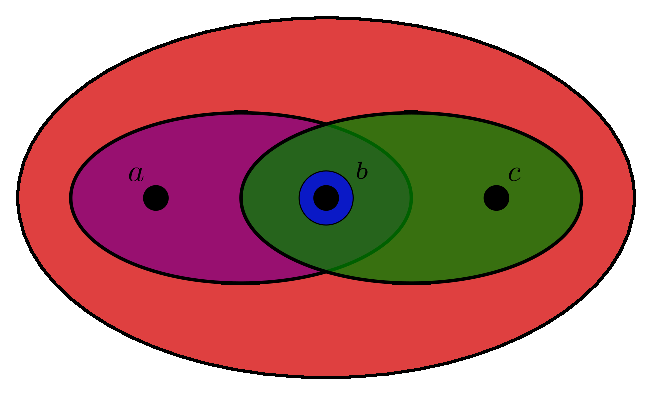
\includegraphics[scale = 0.5]{Figures/Chapter1/non_hausdorff_space.eps}
            \caption{A topology on $\{a,b,c\}$, is not a Hausdorff space.}
            \label{fig_1.8}
        \end{figure}
        figure \ref{fig1.8}, and define the sequence $\{x_n\}$ by  $x_n=b$ for all
        $n \in \Z^+$. The neighborhoods of  $a$, $b$, and $c$ are
        $U_a=\{a,b\}$,  $U_b=\{b\}$, and  $U_c=\{b,c\}$. Now let $N>0$, then we see
        that for all  $n \geq N$, that  $b \in U_a$, $b \in U_b$, and $b \in U_c$
        thus  $b$ converges to  $a$ and to  $c$, and itself.

    \item[(2)] Consider the sequence of points $\{\frac{1}{n}\}_{n \in \Z^+}$ of
        $\R$ in the finite complement topology. Then for any neighborhood  of
        $x \in \R$, which is of the form $\com{\R}{U}$, there are finitely many
        $\frac{1}{n}$ not included. Thus we get that $\lim{\frac{1}{n}}=x$ as $n
        \rightarrow \infty$ for all $x \in \R$.
    \end{enumerate}
\end{example}

\begin{definition}
    A topological space $X$ is called a \textbf{Hausdorff space} if for each
    pair of distinct points  $xy$ , and $y$, there are neighborhoods $U$
    and $V$ of $x$ and $y$ respectively such that $U$ and $V$ are disjoint.
\end{definition}

\begin{example}
    The topology of the previous example in figure \ref{fig_1.8} is not a
    Hausdorff space.
\end{example}

\begin{theorem}\label{1.6.8}
    Every finite point set in a Hausdorff space is closed.
\end{theorem}
\begin{proof}
    Let $X$ be a Hausdorff space, and let  $x_0 \in X$. We have that
    $\cl{\{x_0\}}=\bigcap_{\{x_0\} \in U}{U}$. Now let $x \neq x_0 \in X$.
    Since $x \otin \{x_0\}$, and $X$ is Hausdorff, the intersections of the
    neighborhoods of $x$ and  $ x_0$ is empty, thus $x \notin \cl{\{x_0\}}$,
    therefore $\cl{\{x_0\}}=\{x_0\}$.

    We can then extend this proof to finite point sets of size $n$ by induction.
\end{proof}

Now the condition that finite point sets be closed need not depend on whether or
not $X$ is a Hausdorff space. In fact, we can assume the following for some
topological spaces.

\begin{axiom}[The $T_1$ Axiom]\label{axm1.6.1}
    In any topological space, every finite point set of $X$ is closed.
\end{axiom}

\begin{theorem}\label{1.6.9}
    Let $X$ be a topological space satisfying the $ T_1$ axiom, and let $A
    \subseteq X$. Then a point  $x$ is a limit point of  $A$ if and only if
    every neighborhood of  $x$ contains infinitely many points of  $A$.
\end{theorem}
\begin{proof}
    Let $U_x$ be a neighborhood of  $x$. If  $U_x$ intersects $A$ at infinitely
    many points of  $A$, then it intersects  $A$ at a point distinct from  $x$,
    thus  $x$ is a limit point of  $A$.

    Conversely suppose that  $x$ is a limit point of  $A$, and let  $U_x \cap A$
    be finite, then  $U_x \cap (\com{A}{\{x\}})$ is also  finite. Now let
    $U_x \cap (\com{A}{\{x\}})=\{x_1, \dots x_m\}$. By the $T_1$ axiom,
    $\{x_1, \dots, x_m\}$ is closed, so $\com{X}{\{x_1, \dots, x_m\}}$ is open,
    thus $U_x \cap (\com{X}{\{x_1, \dots, x_m\}})$ is a neighborhood of $x$ that
    does not intersect  $\com{A}{\{x\}}$, which contradicts that  $x$ is a
    limit point.
\end{proof}

\begin{theorem}\label{1.6.11}
    If $X$ is a Hausdorff space, then a sequence of points of  $X$ converges to
    at most one point in  $X$.
\end{theorem}
\begin{proof}
    Let $\{x_n\}$ be a sequence of points converging to $x$, and let  $y \neq x$
    and let  $U_x$ and  $U_y$ be neighborhoods of  $x$ and  $y$ respectively.
    Then $U_x \cap U_y = \emptyset$. Now since  $\{x_n\}$ converges to  $x$, we
    have that for $N>0$, $x_n \in U_x$ whenever $n \geq N$. Then $x_n \notin
    U_y$, and so  $\{x_n\}$ cannot converge to  $y$.
\end{proof}

\begin{definition}
    Let $\{x_n\}$ be a sequence in a Hausdorff space  $X$. If  $\{x_n\}$
    converges to a point $x \in X$, we call  $x$ the \textbf{limit} of
    $\{x_n\}$ as $n$  \textbf{approaches} $\infty$ and we write $\lim_{n
    \rightarrow \infty}{x_n}=x$ or $\{x_n\} \rightarrow x$ as $n \rightarrow
    \infty$.
\end{definition}

\begin{theorem}\label{1.6.12}
    The following are true:
        \begin{enumerate}
            \item[(1)] Every simply oredered set under the order topology is
                Hausdorff.

            \item[(2)] The product of two Hausdorff spaces is Hausdorff.

            \item[(3)] The subspace of a Hausdorff space is Hausdorff.
        \end{enumerate}
\end{theorem}
\begin{proof}
    \begin{enumerate}
        \item[(1)] Let $X$ be an ordered set under the order topology. Take  $x,y \in
            X$ distinct, and suppose without loss of generality that $x<y$. Then
            consider the neighborhoods  $(-\infty,x]$ and  $[y,\infty)$ of  $x$
            and  $y$ respectively. Then  $(-\infty,x] \cap
            [y,\infty)=\emptyset$.

        \item[(2)] Let $X$ and  $Y$ be Hausdorff, and consider  $X \times Y$ in the
            product topology. Let  $ x_1 \times y_1$ and $ x_2 \times y_2$ be
            distinct points, and let $U_{x_1}$, $U_{x_2}$, $V_{y_1}$ and
            $V_{y_2}$ be basis elements of $ x_1$, $ x_2$, $y_1$, and $y_2$
            respectively. Then they are neighborhoods of those elements
            respectively.

            Now we have that $U_{x_1} \times V_{y_1}$ and $U_{x_2} \times
            V_{y_2}$ are basis elements of $ x_1 \times y_1$ and $ x_2 \times
            y_2$, respectively, and hence neighborhoods of those elements
            respectively.Then we have $(U_{x_1} \times V_{y_1}) \cap (U_{x_2} \times
            V_{y_2})=(U_{x_1} \cap U_{x_2}) \times (V_{y_1} \cap V_{y_2}) = \emptyset
            \times \emptyset =\emptyset$.

        \item[(3)] Let $X$ be Hausdorff, and let  $Y$ be a subspace of  $X$. Let  $x_1$
            and $x_2$ be distinct points, and let  $U_{x_1}$ and $U_{x_2}$ be
            their neighborhoods. Since $Y$ is open in  $X$, then so are  $Y \cap
            U_{x_1}$ and $Y \cap U_{x_2}$, so they are also neighborhoods of $
            x_1$ and $ x_2$ respectively. Then $(Y \cap U_{x_1}) \cap
            (Y \cap U_{x_2})=Y \cap (U_{x_1} \cap
            U_{x_2})=\emptyset$.
    \end{enumerate}
\end{proof}

\begin{definition}
    For any set $X$, we define the \textbf{diagonal} of $X$ to be the set
    \begin{equation}
        \Delta(X)=\{x \times x : x \in X\}
    \end{equation}
\end{definition}

\begin{theorem}\label{1.6.13}
    A topological space $X$ is Hausdorff if, and only if the diagonal
    $\Delta(X)$ is closed.
\end{theorem}
\begin{proof}
    Suppose that $X$ is Hausdorff, then for any  $x,y \in X$ distinct, there are
    neighborhoods $U_x$ and  $U_y$ of $x$ and  $y$ respectively with $U_x$ and
    $V_y$ disjoint. Notice then that  $\com{X}{U_x}$ and $\com{X}{V_y}$ are
    closed in $X$, hence  $\com{(X \times X)}{(U_x \times V_y)}$ is also closed.
    Now, since $x \neq y$ in the neighborhood of $U_x \times V_y$ we get that
    the intersection:
    \begin{equation*}
        \bigcap_{x,y \in X}{\com{X \times X}{U_x \times V_y}}=\Delta(X)
    \end{equation*}
    So $\Delta(X)$ is closed.

    Conversely, suppose that $\Delta(X)$ is closed. Then $\com{(X \times
X)}{\Delta(X)}=\{x \times y : x \neq y\}$ is open. Now, let $U \times V$ be a
neighborhood for some  $x \times y \in \com{(X \times X)}{\Delta(X)}$ as a
subspace of $X \times X$. Then  $U$ is a neigborhood for  $x$ and  $V$ is a
neighborhood for  $Y$. Now, if  $U \cap V \neq \emptyset$, there is some  $z \in
U$ and  $z \in V$, so that  $z \times z \in U \times V$. But  $U \times V$ is a
neighborhood contained in  $\com{(X \times X)}{\Delta(X)}$, which contradicts $z
\times z \in U \times V$. Therefore,  $U$ and  $V$ must be disjoint, which makes
 $X$ into a Hausdorff space.
\end{proof}
 We conclude this section by looking at another characteristic of sets in
 topological spaces, closely related to the interior and closure of sets.

 \begin{definition}
     Let $X$ be a topological space, and  $A \subseteq X$. We define the
     \textbf{boundry} of $A$
     \begin{equation}
         \partial{A}=\cl{A} \cap \cl{(\com{X}{A})}
     \end{equation}
 \end{definition}

\begin{figure}[h]
    \centering
    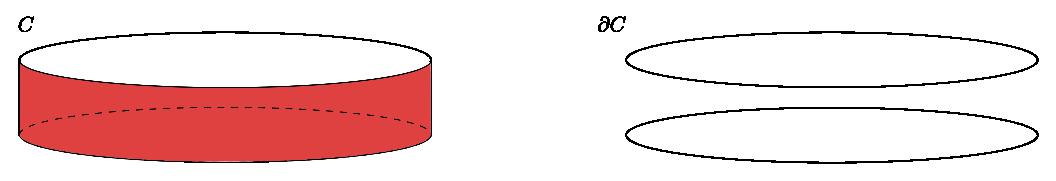
\includegraphics[scale=0.5]{Figures/Chapter1/boundry_cylinder.eps}
    \caption{The boundryd $\partial{C}$ of a cylinder $C$ whose interior is
    empty is the disjouint union of the two circles that enclose $C$.}
    \label{fig_1.9}
\end{figure}

\begin{example}\label{1.18}
    The following are true about the boundry:
    \begin{enumerate}
        \item[(1)] $\Int{A}$ and $\partial{A}$ are disjoint and $\cl{A}=\Int{A}
            \cup \partial{A}$.

        \item[(2)] If $A$ is open and closed, then $\partial{A}=\emptyset$.

        \item[(3)] If $A$ is open, then  $\partial{A}=\com{\cl{A}}{A}$.
    \end{enumerate}
\end{example}

\begin{figure}[h]
    \centering
    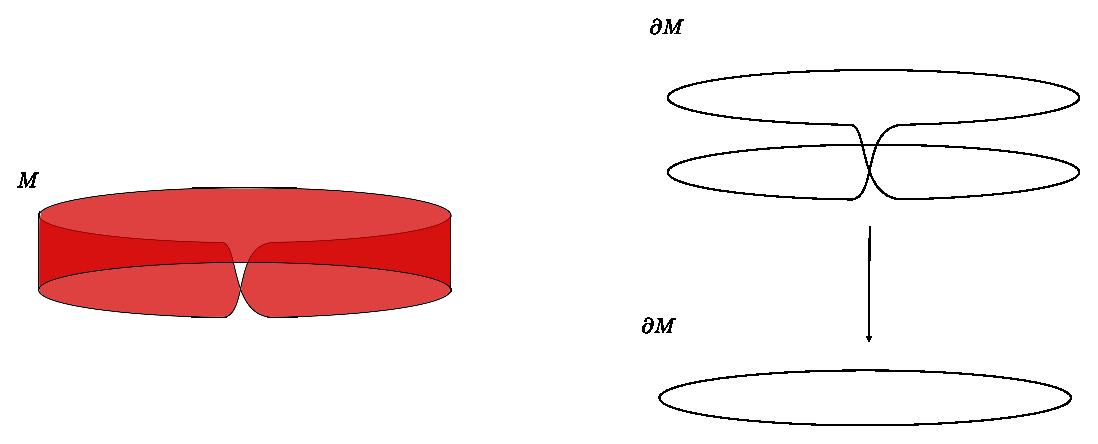
\includegraphics[scale=0.5]{Figures/Chapter1/boundry_mobius.eps}
    \caption{The M\"obius strip is a well known example of an object with only
    one side. It can be recreated by taking a thin strip of tape, twisting it,
    and then gluing the ends together. It can be show that the boundry of a
    M\"obius strip is homeomorphic to a circle.}
    \label{fig_1.9}
\end{figure}
